To evaluate the final system, we did a quantitative evaluation based on experimentation. We set up several scenarios taking place at ITU. The results of each scenario is presented and interpreted below. Due to the issue mentioned in the first scenario we chose to test the prediction implementation seperately.

\section{Scenario 1}
\label{sec:scen1}
The purpose of this scenario is to test if the Raspberry Pi analyses the image and sends the correct data to the server. 

Three webcameras are each connected to a Raspberry Pi and records the Atrium of ITU. 

A person walks across the monitored areas. 

First, three exit areas are manually set in one area by sending requests to the server containing the coordinates of the desired exit points. We perform a probability request by providing a room id and the id of an occupant stored in the database. The Raspberry Pi sends data about the person's position and room to the server which stores it in the database. 

\begin{enumerate}
\item The coordinates of the person are calculated and stored correctly while the id of the object is mistranslated and is stored incorrectly. 
\item The server returns a set of probabilities to each exit. 
\end{enumerate}

The outcome of result 1 indicates that the server does not maintain a link between each coordinate, thus, the complete path of the person is not stored. This is crucial since data about a person's path is essential in calculating probabilities. This is shown in the outcome of result 2 containing inaccurate probabilities. This is because the lack of path information prevents the probability calculations from using the previous position of an occupant, as well as the entrance area of the occupant. Ultimately, this made us choose to test the prediction model in a seperate environment. The tests are described in section \ref{eval_prediction}.

\section{Scenario 2}
The purpose of this scenario is to test the image analysis when multiple people are present in the monitored area.

A webcamera is connected to a Raspberry Pi and records the Atrium of ITU.

Multiple people enter and exit the monitored area.

\begin{enumerate}
\item Several people are moving while a keeping a distance of 2 or more meters of each other and are interpreted as seperate occupants with different ids.
\item Several people are moving while a keeping a distance of less than 2 meters of each other and are interpreted as one occupant with the same id.
\item Two people are entering the monitored area and are initially interpreted as seperate occupants. They intersect and split and are interpreted as new occupants.
\end{enumerate}

The outcome of result 2 and 3 is partly due to the camera placement and because the differentiation of the occupants is only based on the positions. 

\section{Prediction model}
\label{eval_prediction}
Due to the issue mentioned in section \ref{sec:scen1}, we continued the testing of the prediction model in a separate program allowing for easy setup of a desired scenario testing various aspects of the prediction model. The program is implemented in C\# and uses the same logic as the Java implementation. Figure \ref{fig:pred_c} shows an image of the program where each cell is marked with the activity value. The purpose of this setup is to test whether the implemented rule sets have an effect.
\begin{figure}[htb]
	\centering
	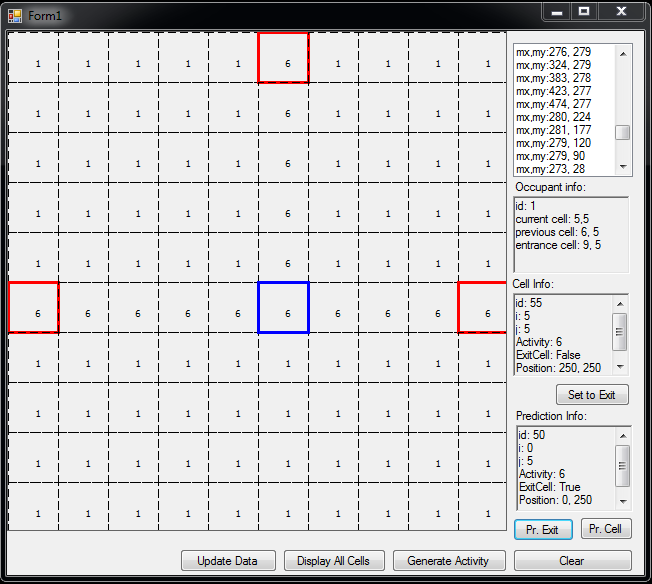
\includegraphics{prediction_figures/prediction_csharp}
	\caption{Screenshot of the prediction test program.}
	\label{fig:pred_c}
\end{figure}
The image depicts a scenario where the occupant entered at the right exit and moving left. He is currently positioned at the blue square. By pressing the "Pr. Exit" button the program will perform the calculation. The left cell is the predicted exit. The probabilities for each exit are only printed to the console in the test program. The results are:
\begin{verbatim}
    Exit at: 0 , 5 , prob=0,3576
    Exit at: 5 , 0 , prob=0,3494
    Exit at: 9 , 5 , prob=0,2930
\end{verbatim}
Since each activity value is the same along the paths to each exit, the rules must have had an effect. The occupant is most likely to exit to the left because he came from the right. He is least likely to exit to the right even though he is positioned closer because this exit serves as his entrance. Moving the occupant one cell to the left increases the probability that he will exit to the left to 0,4935. This is intended as the distance to the left exit decreases. Increasing the activity value in the cells along the path to the topmost exit to 7 increase the probability to the topmost exit to 0,3607, making it the predicted exit when the occupant is positioned at the original location. 